% !TEX root = lnp.tex

%%%%%
%%%%% Commands for chapter 
%%%%%


%%%%% isotope notation
\newcommand{\nuc}[2]{\ensuremath{^{#2}\mathrm{#1}}}

\newcommand{\nn}{\ensuremath{\bar{n}}}

%%%%% observable / interaction name shortcuts
\newcommand{\NNNLO}{N$^3$LO}
\newcommand{\NNLO}{NNLO}
\newcommand{\NNLOsat}{$\text{NNLO}_\text{sat}$}
\newcommand{\Vlowk}{\ensuremath{V_{\text{low-k}}}}
\newcommand{\Vsrg}{\ensuremath{V_{\text{SRG}}}}

\newcommand{\Trel}{\ensuremath{\TO_\text{rel}}}
\newcommand{\Tint}{\ensuremath{\TO_\text{int}}}
\newcommand{\Tcm}{\ensuremath{\TO_\text{cm}}}
\newcommand{\Tpair}{\ensuremath{\TO_\text{pair}}}
\newcommand{\Hint}{\ensuremath{\HO_\text{int}}}
\newcommand{\Epair}{\ensuremath{E_\text{pair}}}
\newcommand{\Rch}{\ensuremath{R_\text{ch}}}
\newcommand{\Hfinal}{\ensuremath{\mkern 3mu\overline{\mkern-3muH}}}

%%%%% flow parameters
\newcommand{\lambdaSRG}{\ensuremath{\lambda}}

%%%%% basis truncations
\newcommand{\aHO}{\ensuremath{a_{\text{HO}}}}
\newcommand{\hw}{\ensuremath{\hbar\omega}}
\newcommand{\eMax}{\ensuremath{e_{\text{max}}}}
\newcommand{\lMax}{\ensuremath{l_{\text{max}}}}
\newcommand{\EMax}{\ensuremath{E_{3\text{max}}}}
\newcommand{\Nmax}{\ensuremath{N_\text{max}}}

%%%%% units
% \newcommand{\fm}{\ensuremath{\,\text{fm}}}
\newcommand{\fmi}{\ensuremath{\,\text{fm}^{-1}}}
\newcommand{\AMeV}{\ensuremath{\,\text{AMeV}}}
\newcommand{\keV}{\ensuremath{\,\text{keV}}}
% \newcommand{\MeV}{\ensuremath{\,\text{MeV}}}
\newcommand{\MeVi}{\ensuremath{\,\text{MeV}^{-1}}}
\newcommand{\eV}{\ensuremath{\,\text{eV}}}
% \newcommand{\GeV}{\ensuremath{\,\text{GeV}}}

%%%%% states and operators
% \newcommand{\ket}[1]{\ensuremath{\,|{#1}\rangle}}
% \newcommand{\braket}[2]{\ensuremath{\langle{#1}|{#2}\rangle}}
\newcommand{\matrixe}[3]{\ensuremath{\langle{#1}|\,{#2}\,|{#3}\rangle}}
\newcommand{\rmatrixe}[3]{\ensuremath{ \abrapar {#1} \big|\big| \,{#2}\, \big|\big| {#3} \aketpar }}


\newcommand{\op}[1]{\ensuremath{\hat{#1}}}
\newcommand{\adj}[1]{\ensuremath{#1}^\dag}
% \newcommand{\vec}[1]{\enusremath{\mathbf{#1}}}

\newcommand{\aO}{\ensuremath{a}}
\newcommand{\aaO}{\ensuremath{\adj{a}}}

\newcommand{\HO}{\op{H}}
\newcommand{\TO}{\op{T}}
\newcommand{\VO}{\op{V}}

\newcommand{\kOV}{\op{\vec{k}}}
\newcommand{\pOV}{\op{\vec{p}}}
\newcommand{\qOV}{\op{\vec{q}}}


%%%%% normal ordering
\newcommand{\nord}[1]{\left\{#1\right\}}


%%%%% commutator
\newcommand{\comm}[2]{\ensuremath{[{#1},{#2}]}}
\newcommand{\acomm}[2]{\ensuremath{ \big\{ {#1}, {#2} \big\} }}

%%%%% editorial
\newcommand{\tbd}[1]{{\color{red}#1}}
\newcommand{\ed}[1]{{\color{blue}#1}}


%%%%% aliases for the figure and program directories
% this will be helpful if we change the  numbering
\newcommand{\fdir}{Chapter10-figures}
\newcommand{\pdir}{Chapter10-programs}


%%%%%
%%%%% Subject matter
%%%%%

\title{In-Medium Similarity Renormalization Group Approach to the Nuclear Many-Body Problem}

\author{Scott K.~Bogner, Heiko Hergert, Justin Lietz, Titus D.~Morris, Sam Novario, Nathan Parzuchowski, and Fei Yuan}
\institute{Scott Bogner  \at Department of Physics and Astronomy and National Superconducting Cyclotron Laboratory, Michigan State University, East Lansing, Michigan USA, \email{bogner@nscl.msu.edu}, \and Heiko Hergert  \at Department of Physics and Astronomy and National Superconducting Cyclotron Laboratory, Michigan State University, East Lansing, Michigan USA, \email{hergert@nscl.msu.edu}, \and Justin G.~Lietz \at Department of Physics and Astronomy and National Superconducting Cyclotron Laboratory, Michigan State University, East Lansing, Michigan,  USA, \email{lietz@nscl.msu.edu}, \and Titus Morris  \at Department of Physics and Astronomy and National Superconducting Cyclotron Laboratory, Michigan State University, East Lansing, Michigan USA, \email{morrist@nscl.msu.edu}, \and Samuel Novario \at Department of Physics and Astronomy and National Superconducting Cyclotron Laboratory, Michigan State University, East Lansing, Michigan,  USA, \email{novarios@nscl.msu.edu},\and Nathan Parzuchowski  \at Department of Physics and Astronomy and National Superconducting Cyclotron Laboratory, Michigan State University, East Lansing, Michigan USA, \email{parzuchowski@frib.msu.edu}, \and Fei Yuan  \at Department of Physics and Astronomy and National Superconducting Cyclotron Laboratory, Michigan State University, East Lansing, Michigan USA, \email{yuan@nscl.msu.edu}}
\maketitle
\abstract{We present applications  of the In-Medium Similarity
Renormalization Group (IM-SRG) method to studies of infinite nuclear matter. 
The IM-SRG method employs a continuous unitary transformation of the
many-body Hamiltonian to decouple the ground state from all
excitations, thereby solving the many-body problem. Starting from a
pedagogical introduction of the underlying concepts, the IM-SRG flow 
equations are developed and we study different IM-SRG generators that
achieve the desired decoupling, and how they affect the details of the IM-SRG results. We compare with the coupled cluster theory results of
chapter \ref{chapter:cc}, the Monte Carlo results of chapter \ref{chapter:qmc} and the Green's function results of chapter \ref{chapter:scgf}.}

\section{Introduction}


\tbd{[Rework the beginning]}
An \emph{ab initio} approach attempts to describe nuclear
structure and dynamics based on fundamental degrees of freedom and their
interactions. In the Standard Model, the fundamental theory of strong
interactions is Quantum Chromodynamics (QCD), but a description of nuclear 
observables on the level of quarks and gluons is not feasible, 
except for the lightest few-nucleon systems (see, e.g., \cite{Detmold:2015xw}).
Instead, we start from nuclear interactions that describe low-energy QCD observables in the $NN$ and $3N$
systems, like scattering data or binding energies. Nowadays, such interactions 
are derived in Chiral Effective Field Theory (EFT),
which provides a constructive framework and organizational hierarchy
for $NN$, $3N$, and higher many-nucleon forces, as well as consistent
electroweak operators (see, e.g., \cite{Epelbaum:2009ve,Machleidt:2011bh,Epelbaum:2015gf,Entem:2015qf,Gezerlis:2014zr,Lynn:2015eu,Pastore:2009zr,Pastore:2011dq,Piarulli:2013vn,Kolling:2009yq,Kolling:2011bh}).
Since Chiral EFT is a low-momentum expansion, high-momentum (short-range)
physics is not explicitly resolved by the theory, but parametrized
by the so-called low-energy constants (LECs). 

\tbd{[Hierarchy of theories]}
In principle, the LECs can be determined by matching calculations of
the same observables in chiral EFT and (Lattice) QCD in the overlap
region of the two theories. Since such a calculation is currently not 
feasible, they are
fit to experimental data, typically in the $\pi{}N$, $NN$, and $3N$ sectors. 
Recently, Ekstr\"om \emph{et al.} have developed an optimization protocol
for chiral interactions that gives up on the reductionist approach of
fixing the LECs in the few-nucleon system, and includes certain many-body
data in the fit as well. The chosen many-body data, e.g., selected radii, are 
chosen in order improve the deficient saturation behavior of chiral interactions 
that are used as input for nuclear many-body calculations. The first interaction
optimized with this protocol is \NNLOsat{} \cite{Ekstrom:2015fk}, which is
able to accurately describe the ground-state energies and charge radii of 
$\nuc{Ca}{40,48}$ at the same time. Following 
the same philosophy but not the same approach, Shirokov \emph{et al.} have 
produced Daejeon16, a softened chiral $NN$ interaction that has been tuned 
for the description of light nuclei without explicit $3N$ forces, to facilitate
Full CI (FCI) calculations \cite{Shirokov:2004fe,Shirokov:2005bv,Shirokov:2007by,Shirokov:2016wo}.

Renormalization group (RG) methods are natural companions for
EFTs, because they make it possible to smoothly connect theories with 
different resolution scales and degrees of freedom. Since they 
were introduced in low-energy nuclear physics around the start 
of the millennium \cite{Bogner:2003os,Bogner:2007od,Bogner:2010pq,Furnstahl:2013zt}, 
they have provided a systematic framework for formalizing many ideas on the 
renormalization of nuclear interactions and many-body effects that had been 
discussed in the nuclear structure community since the 1950s. For instance,
soft and hard-core $NN$ interactions can reproduce scattering data equally
well, but have significantly different saturation properties, which caused
the community to move away from the former in the 1970s (see, e.g., \cite{Bethe:1971qf}).
What was missing at that time was the recognition of the intricate link
between the off-shell $NN$ interaction and $3N$ forces that was formally
demonstrated for the first time by Polyzou and Gl\"ockle in 1990 \cite{Polyzou:1990fk}.
From the modern RG perspective, soft- and hard-core interactions emerge
as representations of low-energy QCD at different resolution scales, 
and the dialing of the resolution scale necessarily leads to induced
$3N$ forces, in such a way that observables (including saturation
properties) remain invariant under the RG flow (see section \ref{sec:srg} 
and \cite{Bogner:2010pq,Furnstahl:2013zt}). In conjunction, chiral EFT
and nuclear RG applications demonstrate that one cannot treat the $NN, 3N, \ldots$
sectors in isolation from each other.

\tbd{[Contrary to G-matrix....]}In the SRG and other
modern RG approaches, low- and high-momentum physics are decoupled properly,
and the resulting low-momentum $NN+3N$ interactions are indeed perturbative
 \cite{Bogner:2006qf,Bogner:2010pq}. For such interactions, results from 
finite-order many-body perturbation theory (MBPT) are in good agreement 
with non-perturbative results if the expansion is based on a Hartree-Fock 
reference state \cite{Tichai:2016vl,Roth:2010ys}.

Of course, low-momentum $NN+3N$ interactions are well-suited inputs not
just for MBPT, but for all methods that work in truncated configuration
spaces. The decoupling of low- and high-momentum modes of the interaction
leads to a greatly improved convergence behavior, which in turn extends 
the range of nuclei a many-body method can be applied to. With SRG-evolved
interactions, the No-Core Shell Model (NCSM) and related FCI methods can
be extended into the lower $sd-$shell 
\cite{Barrett:2013oq,Jurgenson:2013fk,Hergert:2013ij,Roth:2014fk}, and 
methods with systematic many-body truncations like Coupled Cluster (CC)
are nowadays applied to nuclei as heavy as tin \cite{Binder:2014fk,Hagen:2014ve,Hagen:2016rb}.

In the examples discussed so far, the SRG has been used to ``pre-process''
free-space interactions that serve as input for nuclear many-body 
calculations. There is no reason why the idea of decoupling energy 
(or momentum) scales should not be useful for the treatment of a
strongly interacting many-body system like the nucleus as well. This
consideration, then, leads us to the concept of the In-Medium SRG
(IM-SRG) \cite{Tsukiyama:2011uq,Hergert:2013mi,Hergert:2016jk}. In a 
nutshell, we want to use SRG-like flow equations to 
decouple physics at different excitation energy scales of the nucleus, 
and render the Hamiltonian matrix in configuration space block or 
band diagonal in the process. This can also be viewed as a re-organization 
of the many-body expansion, in which correlations that are described 
explicitly by the configuration space are absorbed into an 
\emph{RG-improved} Hamiltonian. With an appropriately chosen decoupling 
strategy, it is even possible to extract eigenvalues and eigenstates
of the nuclear Hamiltonian, and therefore, the IM-SRG qualifies as an 
\emph{ab initio} method for solving quantum many-body problems.


The idea of using flow equations to solve quantum many-body problems
was already discussed in Wegner's initial work on the SRG \cite{Wegner:1994dk} 
(also see \cite{Kehrein:2006kx} and references therein). In the 
solid-state physics literature, the approach is also known as 
continuous unitary transformation (CUT) theory, see  
\cite{Heidbrink:2002kx,Drescher:2011kx,Krull:2012bs,Fauseweh:2013zv,Krones:2015ft}.
When we discuss our decoupling strategies for the nuclear many-body
problem, it will become evident that the IM-SRG is related to CC 
\cite{Shavitt:2009,Hagen:2014ve}, canonical transformation theory (CT) 
\cite{White:2002fk,Yanai:2006uq,Yanai:2007kx}, and the Irreducible (or
Anti-Hermitian) Contracted Schr\"odinger Equation (ICSE) approach 
\cite{Nakatsuji:1976yq,Valdemoro:1987zl,Mukherjee:2001uq,Kutzelnigg:2002kx,
Kutzelnigg:2004vn,Kutzelnigg:2004ys,Mazziotti:2006fk}, and there is
even some overlap with purely variational methods (see section \ref{sec:generators}).
What sets the IM-SRG apart from these methods is that the Hamiltonian 
instead of the wave function is at the center of attention, in the
spirit of RG methodology. This seems to be a trivial distinction, but
there are practical advantages of this viewpoint, e.g., the simultaneous 
decoupling of ground and excited states (see section \ref{sec:decoupling}), 
the avoidance of $N$-representability issues \cite{Mazziotti:2007qe}, and
more. Inspired in part by our work on the IM-SRG in nuclear physics, Evangelista 
and co-workers have recently presented the Driven SRG for \emph{ab initio}
calculations in quantum chemistry, which implements IM-SRG transformations 
in terms of inhomogeneous nonlinear equations rather than flow equations 
\cite{Evangelista:2014rq,Li:2015nq,Li:2016rm,Hannon:2016lp}. 


In this work, we will discuss two distinct implementations of the 
IM-SRG ideas. The first is the so-called Multireference IM-SRG (MR-IM-SRG),
which is designed for calculations of the ground-state properties of 
closed- and open-shell nuclei.  Like most many-body
approaches, it relies on the organization of the many-body basis
in terms of a reference state and its excitations. 
Contrary to approaches like MBPT or FCI, which employ Slater
determinant reference states, the MR-IM-SRG is built for arbitrary
correlated reference states. This gives us the greatest possible
flexibility in the description of correlations: Static correlations,
e.g., due to intrinsic deformation, can be built into the reference
state, while dynamic correlations due to the excitation of nucleon pairs, 
triples, etc. are described by the MR-IM-SRG transformation. 

In the following sections we outline the basic ingredients behind the
SRG method, with an emphasis on applications to infinite nuclear
matter, coupling our final results with those of chapter 8, 9 and
11. The next section presents the essential philosophy of the method,
which in practice means to solve Schr\"odinger's equation for a
many-body system in terms of coupled ordinary differential equations
(ODEs). We present also two simple demonstrations of the SRG method with the true vacuum as reference state. This corresponds in principle to finding all eigenvalues of a matrix by the solution of coupled differential equations (ODEs). 
However, compared with standard eigenvalue solvers, this is a less efficient way of finding the full spectrum of a matrix. 
Moreover, with growing dimensionalities, it becomes quickly impossible to store the matrix elements and solve the coupled ODEs. 
Introducing a reference vacuum as done in chapters 8 and 9, allows us to find approximate solutions to properties  like the  ground state energy and the correlation energy, or selected excited states. This leads us to the
to the in-medium SRG (IM-SRG) approach discussed in this chapter. 
We apply thereafter the IM-SRG approach to the simplified pairing  model (presented in chapter 8) and 
to pure neutron matter. We compare our IM-SRG results to those obtained from coupled cluster theory and many-body perturbation theory of  chapter 8 and quantum Monte Carlo of the previous chapter.  In the final section, we present our conclusions and point  to further
perspectives and research directions.

\section{The Similarity Renormalization Group}

The basic idea of the Similarity Renormalization Group (SRG) method is 
quite general: We want to ``simplify'' our system's Hamiltonian
$\HO(s)$ by means of a continuous unitary transformation that is parametrized
by a one-dimensional parameter $s$,
\begin{equation}\label{eq:cut}
  \hat{H}(s)=\hat{U}(s)\hat{H}(0)\hat{U}^{\dagger}(s)\,.
\end{equation}
Here, $\HO(s=0)$ is the starting Hamiltonian. To specify what we mean by ``simpler'',
it is most useful to think of $\HO$ as a matrix rather than an operator for the
time being --- in practice, we are forced to work with discrete and finite matrix
representations of $\HO$ anyway. As in any quantum mechanical problem, we are 
primarily interested in finding the eigenstates of $\HO$ by diagonalizing its
matrix representation. This task is simplified if we can construct a unitary 
transformation that renders the Hamiltonian more and more diagonal as $s$ 
increases. 



Of course, this idea is very general, and not necessarily related to renormalization.


\tbd{[General Concept, leave nuclear interactions for last subsection, bridge to IM-SRG]}
The Similarity Renormalization Group (SRG) method was first formulated by
Wegner \cite{Wegner:1994dk} and Glazek and Wilson \cite{Glazek:1993il}
to study condensed matter systems and light-front quantum field
theories, respectively.  From a mathematical point of view, the
philosophy behind the SRG is to render the Hamiltonian $\hat{H}(s)$
diagonal via a continuous unitary transformation
\begin{equation}\label{eq:cut}
  \hat{H}(s)=\hat{U}(s)\hat{H}(0)\hat{U}^{\dagger}(s)\,,
\end{equation}
where $H(s=0)$ is the starting Hamiltonian and $s$ denotes the so-called flow
parameter, for reasons that will become apparent shortly. In practice, the demand 
for strict diagonality is usually relaxed to requiring band- or block-diagonality 
of the Hamiltonian matrix in a chosen basis
These specific cases are realized in nuclear
physics applications, where the SRG is used to decouple momentum or
energy scales, and thereby render the nuclear Hamiltonian more
suitable for \emph{ab initio} many-body calculations \cite{Bogner:2007od,Bogner:2010pq,Morris:2015ve,Hergert:2016jk,Hergert:2016ng}.


% We give here a brief overview of the SRG method applied to two simple 
% systems,  a $2\times 2$ matrix and its pertinent eigenvalue problem and 
% the simple pairing model discussed in chapter 8, the latter as a numerical 
% case study in this chapter. 

In the similarity renormalization group (SRG) method, one performs a
continuous sequence of unitary transformations on a Hamiltonian
operator $\hat H$ to evolve it into a more ``amenable'' form, which
generally implies decoupling a small model space of interest from its
complement.  The sequence is parameterized by a continuous variable
$s$ known as the \textit{flow parameter}, which by convention we
define to be $0$ at the beginning of the sequence.  Upon reaching $s$,
the transformed Hamiltonian is given by
\begin{align*}
  \tilde H(s) \equiv \hat U(s) \hat H \hat U(s)
\end{align*}
where $U(s)$ describes the product of all such transformations since $s = 0$.
At every step $s'$, the differential unitary transformation is described by
the exponential of an antihermitian operator $\eta(s)$, known as the
\textit{generator} of the transformation.  When ``integrated'' as a product,
the full transformation $\hat U(s)$ is recovered
\begin{align*}
  \hat U(s) = \lim_{\Delta s' \to 0} \prod_{s' = 0}^{s' = s}
  \mathrm e^{\hat \eta(s') \Delta s'}
\end{align*}
The evolution of the Hamiltonian itself is governed by a differential
equation, commonly referred to as the flow equation:
\begin{gather} \label{eq:imsrgode}
  \frac{d}{d s} \tilde H(s) = [\hat \eta(s), \tilde H(s)]
\end{gather}
which allows $\tilde H(s)$ to be evaluated without explicitly constructing the
full transformation $\hat U(s)$.

 Introducing a flow parameter $s$, there exits a unitary
 transformation $U_s$, such that
\begin{equation}
 \hat{H}_s = U_s^\dagger \hat{H} U_s \equiv \hat{H}^{\rm d}_s + \hat{H}^{\rm od}_s,
\end{equation}
with the relations $U_{s=0} = \mathbf{1}$, and $\hat{H}_{s= 0} =
\hat{H}$.  The transformation $U_s$ is parametrized as
\[
U_s = T_s \exp \left(\int_0^s \! ds'\hat{\eta}_{s'} \right),
\]
where the anti-hermitian operator $\hat{\eta}_s$ serves as generator
of the transformation. With $T_s$ we denote $s$-ordering, which is
defined equivalently to usual time-ordering.  Taking the derivative of
$\hat{H}_s$ with respect to $s$ gives
\begin{equation}
 \frac{d \hat{H}_s}{ds} = \frac{d U_s}{ds}\hat{H} U_s^\dagger + U_s
 \hat{H} \frac{d U_s^\dagger}{ds}.
\label{eq:flowlong}
\end{equation}
Utilizing that for our particular form of $U_s$, we have that 
\begin{equation}
\hat{\eta}_s = \frac{d U_s}{ds} U_s^\dagger = - U_s \frac{d
  U_s^\dagger}{ds} = -\hat{\eta}_s,
\label{eq:eta}
\end{equation} 
we obtain that 
\begin{equation} 
\frac{d \hat{H}_s}{ds} = \hat{\eta}_s \hat{H}_s
- \hat{H}_s \hat{\eta}_s = \left[\hat{\eta}_s, \hat{H}_s \right].
\label{eq:flowEquations}
\end{equation}

This is the key expression of the SRG method, describing the flow
of the Hamiltonian.  The specific unitary transformation is determined
by the choice of $\hat{\eta}_s$.  Through different choices of
$\hat{\eta}_s$, the SRG evolution can be adapted to the features of a
particular problem.
Naively, one could try to solve the flow equation \eqref{eq:flowEquations} by
choosing a suitable basis of the many-body Hilbert space and turning
Eq.~\eqref{eq:flowEquations} into a matrix differential equation, but such an
approach would ultimately amount to a diagonalization of the many-body
Hamiltonian. To make matters worse, implementing the flow means we
would deal with the Hamiltonian's full spectrum rather than just some
extremal eigenvalues that can be extracted efficiently in
state-of-the-art, large-scale large scale diagonalization approaches based on iterative techniques
\cite{Golub:2013le}.

\subsection{Simple demonstration of the SRG method}

In order to get a better understanding of the SRG method, let us first consider  
a simple $2\times 2$ matrix and compare \eqref{eq:flowEquations} with standard diagonalization algorithms like 
Jacobi's rotation method, see for example Ref.~\cite{Golub:2013le}.

We define a  symmetric matrix  $H\in {\mathbb{R}}^{2\times 2}$
\[ 
H = \begin{bmatrix} H_{11} & H_{12} \\ H_{21} & H_{22}\end{bmatrix}. 
\]
The standard Jacobi rotation method allows us to find the eigenvalues via the orthogonal matrix
$\mathbf{U}$ 
\[ 
\mathbf{U} = \begin{bmatrix} c & s \\ -s & c
\end{bmatrix}, 
\]
with $c = \cos \gamma$ and $s = \sin \gamma$. We have then that  $H' = UHU^T$ is diagonal. 

To transform the matrix into one with zero nondiagonal matrix $H'$ we need to solve
\[ 
(H_{22} - H_{11})cs + H_{12}(c^2 - s^2) = 0, 
\]
and using $c^2-s^2 = \cos(2\gamma)$ and $cs = \sin(2\gamma)/2$
this is equivalent with 
\[ \tan(2\gamma) = \frac{2 H_{12}}{H_{11}-H_{22}}. \]
Solving the equation we have
\begin{equation} 
\gamma = \frac{1}{2} \tan^{-1} \left( \frac{2H_{12}}{H_{11}-H_{22}}
\right) + \frac{k\pi}{2}, \quad k=\ldots,-1,0,1,\ldots, \label{eq:0} 
\end{equation}
where $k\pi/2$ is added due to the periodicity of the $\tan$ function.

Note that  $k=0$ gives a diagonal matrix on the form
\begin{equation} 
H'_{k=0} = \begin{bmatrix} \lambda_1 & 0 \\ 0 & \lambda_2 \end{bmatrix},
\label{eq:1} 
\end{equation}
while  $k=1$ changes the diagonal elements  
\begin{equation} 
H'_{k=1} = \begin{bmatrix} \lambda_2 & 0 \\ 0 & \lambda_1 \end{bmatrix}.
\label{eq:2}
\end{equation}

We switch now to the SRG method and 
let $H(s) = T + V(s)$, where $T= \mathrm{diag}(E_1,E_2)$ is diagonal. We want to solve the ordinary differential equations (ODEs) 
for $U(s)$ using the flow parameter $s$. 
We are searching for a transformation 
\[ 
H(s) = U(s)H(0)U(s)^T, 
\]
and we have
\[ 
\frac{d}{ds} H(s) = [\eta(s),H(s)],  \quad \eta(s) = [T,H(s)], 
\]
which gives
\[ 
\frac{d}{ds} U(s) = \eta(s) U(s). 
\]
Note that $\eta(s)^T = -\eta(s)$, that is
\[ 
\eta(s) = \begin{bmatrix} 0 & a(s) \\ -a(s) & 0 \end{bmatrix}. 
\]

To make the link with the Jacobi transformation method
we can parametrize $U(s)$ as
\[ 
U = \begin{bmatrix} \cos(\gamma(s)) & \sin(\gamma(s)) \\ -\sin(\gamma(s)) & \cos(\gamma(s)) \end{bmatrix}. 
\]
Setting up $\eta(s)U(s)$ og $\frac{d}{ds} U(s)$ we arrive at 
\[ 
\frac{d}{ds} \gamma(s) = a(s). 
\]
We apply this to a simple Hamiltonian $H(s)$ (and $T$ and $V(s)$)  defined in term of Pauli matrices  as
\[ 
T = \mathcal{E} I + \Omega \sigma_z, \quad \mathcal{E} = \frac{E_1+ E_2}{2}, \; \Omega = \frac{E_1-E_2}{2}, 
\]
and
\[ 
V(s) = c I \omega_z(s)\sigma_z + \omega_x(s)\sigma_x, 
\]
with $c = (V_{11}+V_{22})/2$, $\omega_z(s) = (V_{11}-V_{22})/2$ and $\omega_x(s) = V_12$. The quantities depend on
$s$. 

We obtain then
\[ \eta(s) = [T, H(s)] = 2\Omega\omega_x(s)\sigma_y, \]
where we have used $\sigma_i\sigma_j = i\epsilon_{ijk}\sigma_k$.
It results in
\[ a(s) = 2\Omega \omega_x(s), \]
and $\gamma(s)$,
\begin{equation} \frac{d}{ds} \gamma(s) = 2\Omega\omega_x(s). \label{eq:3}\end{equation}
We introduce next the  variables $\omega(s)$ and $\theta(s)$ instead of
$\omega_x(s)$ and $\omega_y(s)$. This allows us to write the ODE 
for $\theta(s)$ as
\begin{equation} 
\frac{d}{ds} \theta(s) = -4\Omega\omega \sin(\theta(s)), \label{eq:4}
\end{equation}
and noting that
\[ 
\frac{d}{dx} \ln \tan \frac{x}{2} = \frac{1}{\sin x}, 
\]
we get
\[ 
\tan\left(\frac{\theta(s)}{2}\right) = \exp{-4\Omega\omega s} \tan\left(
  \frac{\theta(0)}{2}\right). 
\]
If $\Omega<0$ ($E_1-E_2<0$) we obtain  $\theta(s)\rightarrow \pi$, and if 
$\Omega>0$ we get  $\theta(s)\rightarrow 0$ and exponential convergence. In a more 
compact form we have
\begin{equation} \theta(s) \rightarrow \pi \vartheta(E_2 - E_1),
  \label{eq:5} \end{equation}
where $\vartheta(x)$ is the  step function.

If we now recall that 
\[ \tan \theta(0) = \frac{2 V_{12}(0) }{[E_1 + V_{11}(0)]- [E_2 +
  V_{22}(0)]},
\]
we can make the link with the Jacobi rotation method. Comparing the  ODE of (\ref{eq:3}) with 
(\ref{eq:4}), we have
\[ \frac{d}{ds} \gamma(s) = -\frac{1}{2} \frac{d}{ds} \theta(s). \]
The initial condition is 
$\gamma(0) = 0$. Integrating we obtain 
\[ \gamma(s) = \frac{1}{2}\theta(0) - \frac{1}{2}\theta(s), \]
and using (\ref{eq:5}) results in 
\[ \gamma(s) \rightarrow \frac{1}{2}\theta(0) -
\frac{\pi}{2}\vartheta(E_2-E_1). \]

From this we see that the flow equation selects the solution of (\ref{eq:0}) with
$k=0$ and $k=-1$, depending on whether  $E_1<E_2$ or $E_2<E_1$.

The flow equation yields $H(s)$ as a continuous function of $s$ and the solution
$H(\infty)$ results in the eigenvalues sorted the same way as
$T = \mathrm{diag}(E_1,E_2)$. The shift $\pi/2$ is connected with this; if $k=0$ in 
(\ref{eq:0}) gives the wrong sequence, we choose $k=-1$ instead!

Let us now apply the above flow equations to the simple pairing model discussed in chapter 8. 

\subsection{The pairing model}
In chapter 8 we presented a simple pairing model, which for the case of four doubly degenerate single-particle states and 
four fermions resulted in the following Hamiltonian matrix
 \[
  H = \begin{bmatrix}
  2\delta -g & -g/2 & -g/2 & -g/2 & -g/2 & 0 \\ -g/2 & 4\delta -g &
  -g/2 & -g/2 & -0 & -g/2 \\ -g/2 & -g/2 & 6\delta -g & 0 & -g/2 &
  -g/2 \\ -g/2 & -g/2 & 0 & 6\delta-g & -g/2 & -g/2 \\ -g/2 & 0 & -g/2
  & -g/2 & 8\delta-g & -g/2 \\ 0 & -g/2 & -g/2 & -g/2 & -g/2 &
  10\delta -g
  \end{bmatrix},
  \]
where $g$ represents the strength of the two-body interaction and $\delta$ is a constant that defines the single-particle energies, see the discussions in chapter 8.  The above Hamiltonian matrix represents the case where no pairs of fermions are broken, resulting in six possible Slater determinats that span the actual model space.

We restate the equations for the various parts of the Hamiltonian here, namely
 \[
  \hat{H}_0 = \delta \sum_{p \sigma} (p-1) a^{\dagger}_{p \sigma} a_{p\sigma},
  \]
for the one-body part
and 
  \[
  \hat{V} = -\frac{1}{2}g \sum_{pq} a^{\dagger}_{p+}a^{\dagger}_{p-}a_{q-}a_{q+},
  \]
for the two-body interaction. The parameters $\delta$ and $g$ are constants.
The single-particle operator $\hat{H}_0$ defines the operator $\hat{T}$ above. We will let $\hat{V}$ have an explicit $s$ dependence. 
In order to solve the coupled ODEs, we use the ODE solver developed by Gordon and Shampine, see for example Ref.~\cite{Shampine:1975qq}.
We follow Wegner's formulation \cite{Wegner:1994dk} in terms of a flow equation
for the Hamiltonian.
The initial  Hamiltonian $\hat{H} = \hat{H}_0 + \hat{V}=\hat{T}+\hat{V}$, where $\hat{H}_0=\hat{T}$ is independent of $s$ and
represents the non-interacting part of the Hamiltonian, is transformed by the 
unitary operator $\hat{U}(s)$ according to
\[ 
\hat{H}(s) = \hat{U}(s)\hat{H}(s=0)\hat{U}(s)^T, 
\]
which results in the equation
\[
  \frac{d\hat{H}(s)}{ds}= [\eta(s),\hat{H}(s)],
\]
with
\[
   \eta(s) = \frac{d\hat{U}(s)}{ds} \hat{U}^\dagger(s) = -\eta^\dagger(s).
\]
Choosing $\eta(s)$ specifies the transformation.
Here we make perhaps the simplest choice \cite{Wegner:1994dk},
\begin{equation}
  \eta(s) =  [\hat{H}_0, \hat{H}(s)]
  \label{eq:choice},
\end{equation}
which gives the flow equation,
\begin{equation}
  \frac{d\hat{H}(s)}{ds}=  [ [\hat{H}_0, \hat{H}(s)], \hat{H}(s)].
  \label{eq:commutator}
\end{equation}
%
Other choices will be discussed below, see also
Refs.~\cite{Hergert:2016jk,Hergert:2016ng,Morris:2016xp} for a detailed discussion of
possible similarity transformations.  The derivative of the
Hamiltonian involves only the potential since we have assumed that
$\hat{H}_0$ is independent of the flow parameter $s$. With a given
basis $k$ the derivative of $\hat{V}$ evolves as, using dimensionless
units and specifying $\hat{V}(s) = \langle k \vert \hat{V}(s) \vert
k'\rangle$, we obtain
\begin{equation} \frac{d(\langle k \vert \hat{V}(s) \vert k'\rangle)}{ds} =- (\varepsilon_k -\varepsilon_{k'} )^2\langle k \vert \hat{V}(s) \vert k'\rangle
    + \sum_{q=0}^{\infty}(\varepsilon_k + \varepsilon_{k'} - 2\varepsilon_{q})\langle k \vert \hat{V}(s) \vert q\rangle\langle q \vert \hat{V}(s) \vert k'\rangle.
      \label{eq:diffeq}
\end{equation}
Here the quantity $\varepsilon_k$ represents the single-particle
energies arising from the non-interacting Hamiltonian. We have assumed
that the basis $k$ forms an eigenbasis for the non-interacting
Hamiltonian $\hat{H}_0$ and we have used the discrete completeness
relation $\sum_{k=0}^{\infty}\vert k \rangle \langle k \vert = 1$.  As
demonstrated below via various numerical examples, when we let $s$
evolve to infinity, the Hamiltonian matrix becomes more and more
diagonal. The code to solve the coupled ODEs is at
\url{https://github.com/ManyBodyPhysics/LectureNotesPhysics/blob/master/doc/src/\pdir/f95} and here we show the function which sets up the derivative of Eq.~(\ref{eq:diffeq}). 
\begin{lstlisting}
! The derative of V as function of a given value of s
! n_total stands for the number of basis function k and v is the potential term
! The terms onebodyenergy  represent the eigenenergies of the non-interacting Hamiltonian H_0
SUBROUTINE derivative(v, dv)
  IMPLICIT NONE
  INTEGER ::  ij, i, j, k
  REAL(8) :: sum, v(:), dv(:), k1, k2, p
  REAL(8), ALLOCATABLE :: vij(:,:)

  ALLOCATE(vij(n_total,n_total)) 
  ij = 0
  DO j = 1, n_total
     DO i = j, n_total
        ij = ij + 1
        vij(i,j) = v(ij)
        vij(j,i) = v(ij)
     ENDDO
  ENDDO
  ij = 0
  DO i = 1, n_total
     k1 = onebodyenergy(i) 
     DO j = i, n_total
        k2 = onebodyenergy(j) 
        ij = ij + 1
        sum = 0_dp
        DO k = 1, n_total
           p = onebodyenergy(k) 
           sum = sum +  (k1+k2-2.0*p)*vij(j,k)*vij(k,i) 
        ENDDO
        dv(ij) =  sum - (k2-k1)*(k2-k1)*vij(j,i)
     ENDDO
  ENDDO
  DEALLOCATE(vij)

END SUBROUTINE derivative
\end{lstlisting}
If we wish to solve the above equations for a nuclear interaction in a
partial wave basis using relative coordinates for the momenta $k$, the explicit equations
become \cite{Bogner:2007od} (with normalization
so that $1 = \frac{2}{\pi}\int_0^\infty|q\rangle q^2\,dq \langle q |$
and in units where $\hbar^2/M = 1$),
%
\begin{equation}
  \frac{d(\langle k \vert \hat{V}(s) \vert k'\rangle)}{ds} =- (k^2 - k'{}^2)^2\langle k \vert \hat{V}(s) \vert k'\rangle
    + \frac{2}{\pi}\int_0^{\infty}q^2dq
      (k^2 + k'{}^2 - 2q^2)\langle k \vert \hat{V}(s) \vert q\rangle\langle q \vert \hat{V}(s) \vert k'\rangle).
\end{equation}
By discretizing the relative momentum space on a grid of Gaussian integration points, 
we obtain a simple (but nonlinear) system of first-order
coupled differential equations,
with the boundary condition that $\langle k \vert \hat{V}(s) \vert k'\rangle$ at the initial
value of $s$ is equal to the initial potential.

Instead of the parameter $s$ which is being evolved to $\infty$, we could define 
the parameter $\lambda \equiv s^{-1/4}$. This parameter  provides a measure of the
spread of the off-diagonal strength when $s$ or $\lambda$ are evolved. The replacement of $s$ by $\lambda$ introduces a multiplicative factor 
of $-2.0/\lambda^3$ in front of the derivative of $\hat{V}$ in the above code sniplet and equations. 

Returning to our pairing problem, in order to run the Fortran program {\em pairing.f90}, which is easily compiled with any available Fortran compiler, the reader needs to specify the relevant input parameters to the pairing model in the file {\em pairing.ini}, displayed here as well
\begin{svgraybox}
\begin{lstlisting}
# Parameters for the simple pairing model code
# It reads the variable names and corresponding values as 
# variable = something
# You can have as many blank lines as you want.   
# to the left is btw the comment sign. But do not change the leftmost
# text string, which is needed by the code to identify which variable
# is used. 

# Dimensionless units are used throughout
# output_run is prefixed to output file for optional printouts, tests etc.
output_run = run_test.dat

# Give the size of the matrix
dimension_matrix = 6


# The values of delta, g, lambda and starting point
value_delta = 1.0
value_g = 0.5
value_lambda = 1.0
value_startpoint = 40.0
\end{lstlisting}
\end{svgraybox}
The program employs $\lambda$ as flow parameter instead of $s$. This means that the starting point for solving the differential equations
should be as large as possible. The smaller the value of $\lambda$, the closer to zero are the non-diagonal matrix elements. 
In the examples here we have chosen 
$g=-0.5$ and the single-particle energy strength $\delta=1$. The resulting exact eigenavalues by diagonalizing the above $6\times 6$ matrix (to six leading digits) are
$1.42705,   3.48610,  11.5572,   9.53081, 7.47926,   5.51955$.

With $\lambda=1$ (or $s=1$), our similarity transformed matrix becomes
\[
\begin{bmatrix}
0.142706E+01 &   -.473950E-02  &   -.213293E-07  &   0.160910E-10  &   -.139603E-10  &   0.127066E-07 \\
    -.473950E-02   &  0.348610E+01  &   -.401318E-02  &   -.274470E-07   &  -.103994E-11  &   0.174969E-10 \\
    -.213293E-07   &  -.401318E-02   &  0.551954E+01   &  -.393739E-05   &  -.278160E-07   &  -.129686E-10 \\
    0.160910E-10   &  -.274470E-07   &  -.393739E-05   &  0.747927E+01   &  -.437695E-02  &   -.204824E-07 \\
    -.139603E-10   &  -.103994E-11   &  -.278160E-07   &  -.437695E-02   &  0.953081E+01  &   -.375229E-02 \\
    0.127066E-07   &  0.174969E-10   &  -.129686E-10   &  -.204824E-07   &  -.375229E-02  &   0.115572E+02
\end{bmatrix}.
\]

\tbd{
With $\lambda=0.1$ (or $s=10$), our similarity transformed matrix becomes
\[
\begin{bmatrix}
0.142705E+01 &   -.413102-179 &   0.000000E+00 &   0.000000E+00 &   0.516773-184 &   -.652307E-07 \\
    -.413102-179   &  0.348610E+01  &   -.556534-177  &   0.000000E+00  &   0.000000E+00  &   -.101304-186 \\
    0.000000E+00   &  -.556534-177  &   0.551955E+01   &  -.119801-173  &   0.000000E+00   &  0.000000E+00 \\
    0.000000E+00   &  0.000000E+00   &  -.119801-173   &  0.747926E+01   &  -.168573-178   &  0.000000E+00 \\
    0.516773-184   &  0.000000E+00   &  0.000000E+00   &  -.168573-178   &  0.953081E+01   &  -.209242-176 \\
    -.652307E-07   &  -.101304-186   &  0.000000E+00   &  0.000000E+00   &  -.209242-176   &  0.115572E+02
\end{bmatrix}.
\]
We see clearly that for $\lambda=0.1$, our eigenvalues are equal to
the exact ones (at the level of six leading digits) and the
non-diagonal matrix are for all practical purposes equal to zero.
}

For the simple pairing model, with modest dimensionalities of the
Hamiltonian matrix, we can solve the flow equations with respect to
the physical vacuum state by setting up the full Hamiltonian matrix,
and solve Eq.~(\ref{eq:flowEquations}) as a set of coupled first-order
differential equations. However, since the size of the problem grows
enormously with the number of particles and the size of the model
space, the applicability of this free-space SRG method is restricted
to comparatively small systems. This leads us to approximations to the
solution of the full set of coupled ODEs. In particular we will here
discuss the in-medium SRG approach, where a new reference vacuum is
introduced (normally defined by the Hartree-Fock state discussed in
chapters 8 and 9). This will allow us to make links with the many-body
methods discussed in chapters 8, 9 and 11. The final part of this
chapter is devoted to a presentation of the in-medium SRG approach and
its applications to the pairing model and infinite nuclear matter.

\subsubsection{Evolution of Nuclear Interactions}
\begin{figure*}[t]
  \begin{center}
    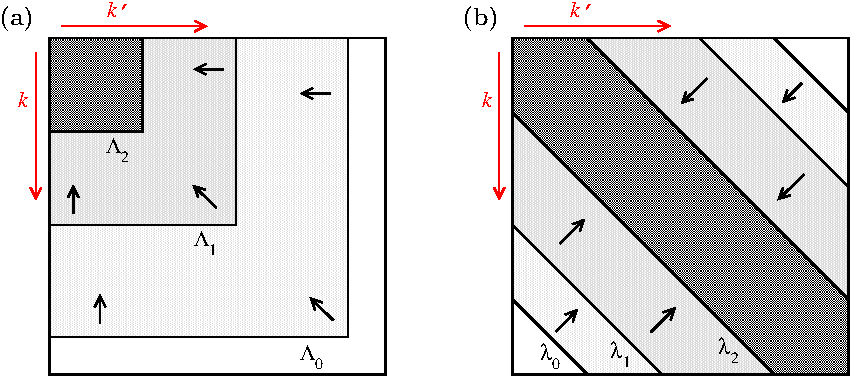
\includegraphics[width=0.9\textwidth]{\fdir/rg_evolution_schematic.pdf}
  \end{center}
  \caption{\label{fig:schematic}Schematic illustration of two types of RG evolution 
    for $NN$ potentials in momentum space: (a) \Vlowk{} running in $\Lambda$, and 
    (b) SRG running in $\lambdaSRG$ (see main text). Here, $k$ and $k'$ denote the 
    relative momenta of the initial and final state, respectively. At each $\Lambda_i$ 
    or $\lambdaSRG_i$, the matrix elements outside of the corresponding 
    blocks or bands are negligible, implying that high- and low-momentum 
    states are decoupled.
  }
\end{figure*}


In figure \ref{fig:schematic}, we show schematic examples of RG evolutions that are applied to
nucleon-nucleon interactions in momentum-space representation. Figure \ref{fig:schematic}(a) 
implements the RG as a decimation: The interaction is evolved to decreasing
cutoff scales $\Lambda_0 > \Lambda_1 > \Lambda_2$, and we end up with a low-momentum interaction
\Vlowk{} that only has non-zero matrix elements between states with initial and final 
relative momenta $k,k'\leq\Lambda$ \cite{Bogner:2003os,Bogner:2010pq}. In contrast, 
figure \ref{fig:schematic}(b) results from a continuous unitary transformation via the flow 
equation \eqref{eq:opflow}, using a Wegner-type generator built from the relative kinetic 
energy in the two-nucleon system:
\begin{equation}\label{eq:def_srg_generator}
  \eta(\lambda) \equiv \Big[\,\frac{\kOV^2}{2\mu}, v(\lambda)\Big]\,.
\end{equation}
Here, $\kOV=\tfrac{1}{2}(\pOV_1-\pOV_2)$, and $\mu$ is the reduced nucleon mass. We have
parametrized the transformation with $\lambdaSRG=s^{-1/4}$, which has the 
dimensions of a momentum (in natural units). As suggested by figure \ref{fig:schematic}(b),
$\lambdaSRG$ is a measure for the ``width'' of the band-diagonal Hamiltonian in momentum 
space, i.e., it controls the scale of momentum transfers between nucleons. Because  
\begin{equation}
  |\qOV|=|\kOV' - \kOV|\lesssim \lambdaSRG
\end{equation}
low- and high-lying momenta are decoupled in a proper RG sense as $\lambdaSRG$ is 
decreased.

The decoupling of low- and high-lying momenta significantly improves the convergence
properties of configuration-space based many-body methods, because it prevents the 
Hamiltonian from scattering nucleon pairs from low to high momentum states. Methods 
like the NCSM or the IM-SRG discussed below yield converged results in much smaller 
many-body Hilbert spaces, which in turn makes it possible to
apply these methods to heavier nuclei \cite{Roth:2011kx,Barrett:2013oq,Jurgenson:2013fk,Roth:2014fk,Hergert:2013ij,Hergert:2013mi,Hergert:2014vn,Hergert:2016jk,Hagen:2010uq,Roth:2012qf,Binder:2013zr,Binder:2014fk,Soma:2011vn,Soma:2013ys,Soma:2014fu,Soma:2014eu}.
 However, this improvement 
comes at a cost, which is best illustrated by considering the Hamiltonian in a 
second-quantized form, assuming only a two-nucleon interaction for simplicity:
\begin{equation}\label{eq:H}
  \Hint = \Trel + V = \frac{1}{4}\sum_{pqrs} \matrixe{pq}{\frac{\kOV_{12}^2}{2\mu}+v_{12}}{rs}\aaO_p\aaO_q\aO_s\aO_r\,.
\end{equation}
If we plug $\Trel$ and $V$ into the commutators in equations \eqref{eq:def_srg_generator} and 
\eqref{eq:opflow}, we obtain
\begin{equation}\label{eq:comm2B_vac}
  \comm{\aaO_i\aaO_j\aO_l\aO_k}{\aaO_p\aaO_q\aO_s\aO_r}=
  \delta_{lp}\aaO_i\aaO_j\aaO_q\aO_s\aO_r\aO_k + \aaO\aaO\aaO\aO\aO\aO
  -\delta_{lp}\delta_{kq}\aaO_i\aaO_j\aO_s\aO_r + \aaO\aaO\aO\aO\,, 
\end{equation}
where the terms with suppressed indices schematically stand for additional two- and
three-body operators. Thus, even if we start from a pure two-body interaction, the SRG 
flow will induce operators of higher rank, i.e., three-, four-, and in general 
up to $A$-nucleon interactions. Of course, these induced interactions 
are only probed if we study an $A$-nucleon system. If we truncate the SRG flow equations
at the two-body level, we preserve the properties of the two-nucleon system, in particular
phase shifts and the deuteron binding energy. A truncation at the three-body level 
ensures the invariance of observables in $A=3$ nuclei, 
e.g.~$\nuc{H}{3}$ and $\nuc{He}{3}$ ground-state energies, and so on. Truncations in the 
SRG flow equation cause a violation of unitarity that manifests as
a (residual) dependence of many-body results on $\lambdaSRG$. By varying this parameter, 
the size of the missing contributions can be assessed (see, e.g., \cite{Bogner:2010pq,
Jurgenson:2009bs,Hebeler:2012ly,Roth:2011kx,Hergert:2013mi,Hergert:2013ij,Binder:2014fk,
Soma:2014eu,Griesshammer:2015dp}).

State-of-the-art SRG evolutions of nuclear interactions are nowadays performed in 
the three-body system, using relative (Jacobi) harmonic oscillator
\cite{Jurgenson:2009bs,Jurgenson:2011zr,Jurgenson:2013fk}, relative momentum plane
wave \cite{Hebeler:2012ly}, or momentum-space hypherspherical harmonics representations 
\cite{Wendt:2013uq}.
Figure \ref{fig:vsrg_momentum} shows an example of the latter, the evolution of 
NN and $3N$ matrix elements of a chiral \NNLO{} interaction by Epelbaum, Gl\"ockle,
and Mei\ss{}ner \cite{Epelbaum:2002nr,Epelbaum:2006mo}, with cutoffs 550/600 MeV. As discussed for our 
schematic example, both the $NN$ and $3N$ interactions become band diagonal and the SRG 
decouples the low- and high-momentum regimes as we evolve to lower values of $\lambdaSRG$. 
In figure \ref{fig:triton}, the same family 
of SRG-evolved interactions is used to calculate the ground-state energy of the triton,
as a function of $\lambdaSRG$. If only the $NN$ part of the chiral interaction is used as 
input, and the SRG generator and flowing Hamiltonian are truncated at the two-body level 
(curve ``NN-only''), the SRG evolution is not unitary in the three-body system. The 
energy exhibits a significant dependence on $\lambdaSRG$, on the order of 5--6\%. If the 
flow equations are truncated at the three-body level instead, induced $3N$ interactions are
properly included and the unitarity of the transformation is restored (\emph{$NN\!+\!3N$-induced}): 
The energy does not change as $\lambdaSRG$ is varied. Finally, the curve \emph{$NN\!+\!3N$-full} 
shows the result for a calculation with initial $NN$ and $3N$ forces, which are consistently 
SRG-evolved at the three-body level. The triton ground-state energy is again invariant 
under the SRG flow, and closely reproduces the experimental value that is used as 
constraint in the adjustment of the $3N$ force's low-energy constants (see, e.g., 
\cite{Epelbaum:2009ve,Machleidt:2011bh,Gazit:2009qf}).

\begin{figure*}[t]
  % \setlength{\unitlength}{\textwidth}
  % \begin{center}
  %   \includegraphics[width=0.95\unitlength]{fig/Vkk_2_and_3_EGM_550_600.png}
  % \end{center}  
  \begin{center}
    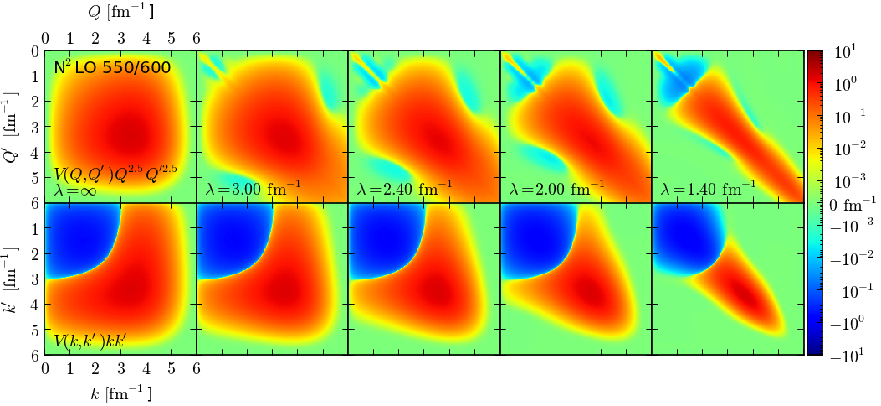
\includegraphics[width=0.95\textwidth]{\fdir/srg_evolution_me.pdf}
  \end{center}    
  \caption{\label{fig:vsrg_momentum}SRG evolution of a chiral \NNLO{} $NN\!+\!3N$
  Hamiltonian with cutoffs $550/600$ MeV \cite{Epelbaum:2002nr,Epelbaum:2006mo}
  in a three-body hyperspherical momentum basis. The figure shows contour
  plots of the matrix elements as a function of $\lambdaSRG$ in the lowest 
  hyperspherical partial wave, both for the $3N$ interaction (top panel)
  and the embedded $NN$ interaction in that
  partial wave (lower panel). See \cite{Wendt:2013ys} for
  additional details. Figure courtesy of K.~Wendt.}
\end{figure*}

\begin{figure*}[t]
  % \setlength{\unitlength}{\textwidth}
  % \begin{center}
  %   \includegraphics[width=0.5\unitlength]{fig/Triton_N2LO.pdf}
  % \end{center}  
  \setlength{\unitlength}{\textwidth}
  \begin{center}
    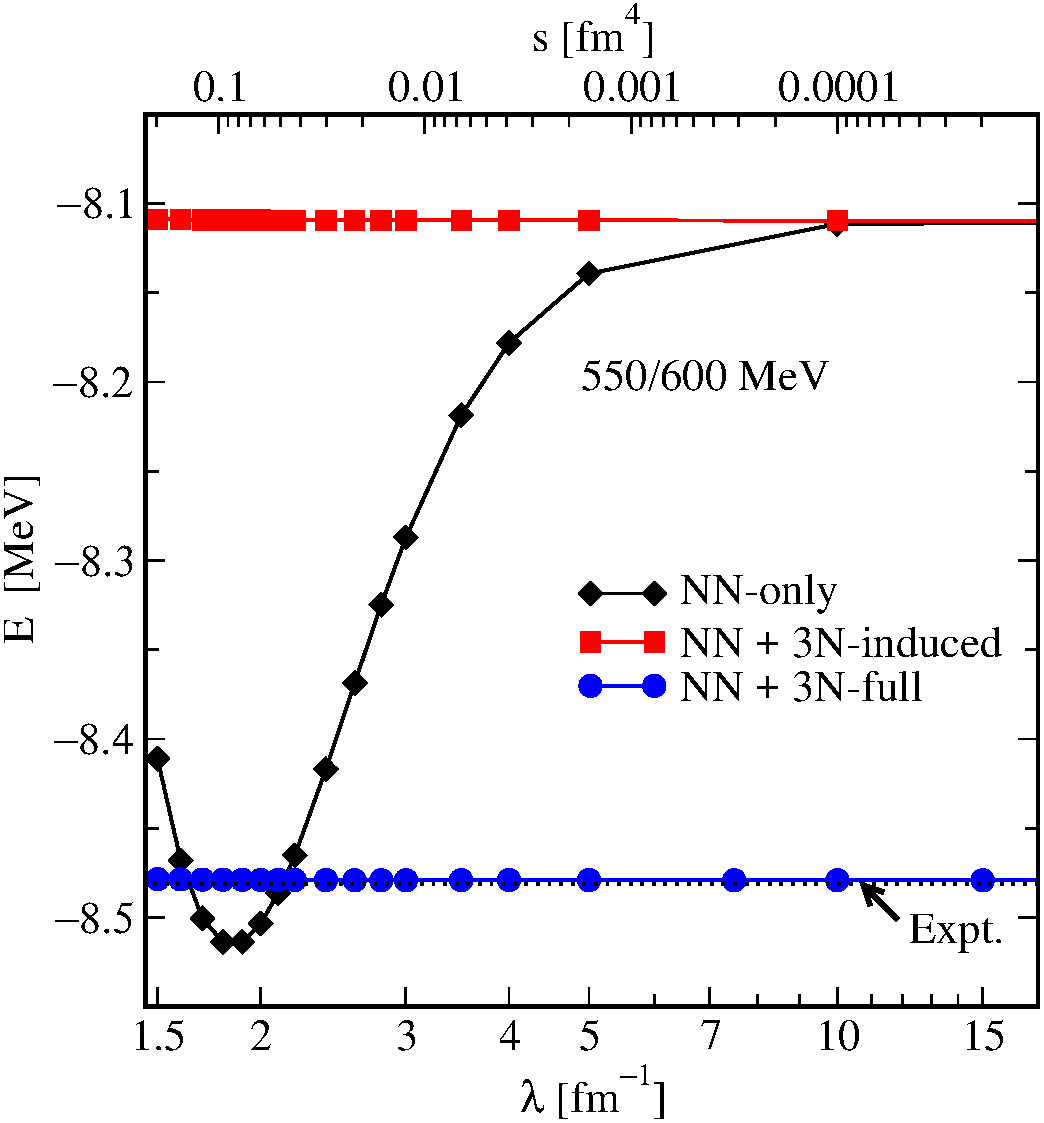
\includegraphics[width=0.5\unitlength]{\fdir/srg_evolution_energy.pdf}
  \end{center}  
  \caption{\label{fig:triton}Ground state energy of $\nuc{H}{3}$ as a function 
  of the flow parameter $\lambdaSRG$ for different initial \NNLO{} $NN\!+\!3N$ interactions
  \cite{Epelbaum:2002nr,Epelbaum:2006mo}. $NN$-only means initial and 
  induced $3N$ interactions are discarded, $NN\!+\!3N$-induced takes only 
  induced $3N$ interactions into account, and $3N$-full contains initial
  $3N$ interactions as well. The black dotted line shows the experimental 
  binding energy \cite{Wang:2012uq}. Figure courtesy of K.~Hebeler.}
\end{figure*}

% Pioneering work on implementing the SRG evolution in the lowest partial 
% waves of the four-body system has been carried out by A.~Calci and 
% co-workers \cite{Calci:2014xy}, again working in Jacobi HO representation.
The SRG flow equations force us to manipulate large sections (or the 
entirety) of the Hamiltonian's spectrum in order to avoid basis 
truncation artifacts (also cf.~\cite{Roth:2014fk,Binder:2014fk})
We may wonder, then, if it is possible to avoid the use of matrix 
representations entirely by solving the operator flow equation 
\eqref{eq:opflow} directly in the algebra of operators. This is the 
strategy that we will explore in the following, which will 
lead us to the formulation of the In-Medium SRG. 

\section{The In-Medium SRG approach}

Instead of performing SRG in free space, the evolution can be done at
finite density, that is directly in the $A$-body system
\cite{Kehrein:2006kx}. This approach has recently been applied very
successfully in nuclear physics, see the recent review of Bogner, Hergert, Morris and collaborators 
\cite{Hergert:2016jk,Hergert:2016ng,Morris:2016xp},
and is called in-medium SRG (IM-SRG). The method allows the evolution
of $3,...,A$-body operators using only two-body machinery, with the
simplifications arising from the use of normal-ordering with respect
to a reference state.

In our case, we assume that the problem can be modelled by a
Hamiltonian containing maximally two-body interaction, as done in chapters 8 and 9. In
second-quantized form, we defined in chapter 8 the normal-ordered Hamiltonian as
\[
\hat{H}_N = \sum_{pq} \langle p|\hat{h}_0|q\rangle a^\dagger_p
a_q+\frac{1}{4} \sum_{pqrs} \langle pq|\hat{v}|rs\rangle a^\dagger_p a^\dagger_q a_s a_r+\sum_{pq,i\le F}
\langle pi|\hat{v}|qi\rangle a^\dagger_p a_q.
\]
In chapter 8 we rewrote the normal-ordered Hamiltonian 
in terms of a new one-body operator and a two-body operator
\[
\hat{H}_N=\hat{F}_N+\hat{V}_N,
\]
with
\[
\hat{F}_N=\sum_{pq} \langle p|\hat{f}|q\rangle a^\dagger_pa_q,
\]
where
\[
\langle p|\hat{f}|q\rangle= \langle p|\hat{h}_0|q\rangle +\sum_{i\le F}
\langle pi|\hat{v}|qi\rangle.
\]
The last term on the right hand side represents a medium modification
to the single-particle Hamiltonian due to the two-body interaction.
Finally, the two-body interaction is given by
\[
\hat{V}_N = \frac{1}{4} \sum_{pqrs} \langle pq|\hat{v}|rs\rangle a^\dagger_p a^\dagger_q a_s a_r.
\]
In the equations below we will use the following shorthand notation for the matrix elements
\[
f_{pq}=\langle p|\hat{f}|q\rangle,
\]
and 
\[
v_{pqrs}= \langle pq|\hat{v}|rs\rangle.
\]
As discussed in chapter 8, the indices $i,j,k,...$
denote hole states below the Fermi level, indices $a,b,c,...$
particles states above the Fermi level, and indices $ p,q,r,...$ can
be used for both particle and hole states. As reference state
$|\Phi_0\rangle$ we choose the ground state of the non-interacting
system, where all single-particle orbitals below the Fermi level are
occupied.

Integrating the flow equations~(\ref{eq:flowEquations}), we face one
of the major challenges of the SRG method, namely the generation of
higher and higher order interaction terms during the flow. With each
evaluation of the commutator, the Hamiltonian gains terms of higher
order, and these induced contributions will in subsequent integration
steps contribute to terms of lower order. In principle, this continues
to infinity. 
To make the method computationally possible, we have to
close the IM-SRG flow equations, suggesting that we are forced to
truncate the equations to a certain order. We choose to truncate both
$\hat{H}_s$ and $\hat{\eta}_s$ at the two-body level, an approach
which is referred to as IM-SRG(2).  This normal-ordered two-body
approximation seems to be sufficient in many cases and has yielded
excellent results for several nuclei
\cite{Tsukiyama:2011uq,Tsukiyama:2012fk,Hergert:2016jk,Hergert:2016ng}.

The
commutator in the flow equations (\ref{eq:flowEquations}) guarantees
that the IM-SRG wave function $U_s^\dagger|\Phi\rangle$ can be
expanded in terms of linked diagrams only
\cite{Shavitt:2009,Hergert:2016jk,Hergert:2016ng}, which suggests that IM-SRG
is size-extensive. Regarding the quality of the SRG results, it means
that the error introduced by truncating the many-body expansions
scales linearly with the number of particles~$N$.

With this
truncation, the generator $\hat{\eta}$ can be written as
\[
\hat{\eta} = \sum_{pq} \eta_{pq}^{(1)} a_p^{\dagger}a_q  +
\frac{1}{4}\sum\limits_{pqrs}\eta_{pqrs}^{(2)} a_p^{\dagger}a_q^{\dagger}a_s
a_r,
\]
where $\eta_{pq}^{(1)}$ and $ \eta_{pqrs}^{(2)}$ are the one- and
two-body elements, respectively. Making use of the permutation
operator $ \hat{P}_{pq}f(p,q) = f(q,p)$ defined in chapter 8, the IM-SRG(2) flow equations
are given by
\begin{align}
\frac{d E_0}{ds} &= \sum_{ia}\left( \eta_{ia}^{(1)}f_{ai} -
\eta_{ai}^{(1)}f_{ia}\right) +
\frac{1}{2}\sum_{ijab}\eta_{ijab}^{(2)}v_{abij},
\label{eq:flow1}\\
\frac{d f_{pq}}{ds}&= \sum_r \left(\eta_{pr}^{(1)}f_{rq} +
\eta_{qr}^{(1)}f_{rp}\right) + \sum_{ia}\left(1-\hat{P}_{ia}\right)\left(
\eta_{ia}^{(1)}v_{apiq} - f_{ia}\eta_{apiq}^{(2)} \right)\notag \\ &
+\frac{1}{2} \sum_{aij} \left(1+\hat{P}_{pq}\right)
\eta_{apij}^{(2)}v_{ijaq} + \frac{1}{2}\sum_{abi}\left(1+\hat{P}_{pq}\right) \eta_{ipab}^{(2)}v_{abiq},
\label{eq:flow2}
\end{align}
\begin{align}
\frac{d v_{pqrs}}{ds} &= \sum_t \left(1-\hat{P}_{pq} \right)\left(
\eta_{pt}^{(1)}v_{tqrs}-f_{pt}\eta_{tqrs}^{(2)}\right)-\sum_t \left(
1-\hat{P}_{rs} \right)\left(\eta_{tr}^{(1)} v_{pqts} - f_{tr}
\eta_{pqts}^{(2)}\right)\notag \\ & +\frac{1}{2}\sum_{ab}
\left(\eta_{pqab}^{(2)} v_{abrs} - v_{pqab}\eta_{abrs}^{(2)}\right)-
\frac{1}{2}\sum_{ij} \left(\eta_{pqij}^{(2)} v_{ijrs} -
v_{pqij}\eta_{ijrs}^{(2)}\right)\notag \\ & -\sum_{ia} \left(1-
\hat{P}_{ia} \right)\left(1-\hat{P}_{pq}\right)\left(1-\hat{P}_{rs} \right)
\eta_{aqis}^{(2)}v_{ipar}.
\label{eq:flow3}
\end{align}
Note that for brevity, we have skipped the explicit $s$-dependence in the equations.

\subsection{Choice of generator}
To determine the specific unitary transformation, one needs to specify
the generator~$\hat{\eta}$. Through different choices, the SRG flow
can be adapted to the features of a particular problem.\\


\paragraph{Wegner's canonical generator}
The original choice, suggested by Wegner \cite{Wegner:1994dk}, reads
\begin{equation} 
\hat{\eta} = \left[ \hat{H}^{\rm d}, \hat{H}^{\rm od} \right] = \left[ \hat{H}^{\rm d}, \hat{H}
  \right].
\label{eq:etaWegner}
\end{equation} 
As commutator between two Hermitian operators, $\hat{\eta}$
fulfils the criterion of antihermiticity and can be shown to suppress
the off-diagonal matrix elements \cite{Kehrein:2006kx}. In general,
matrix elements far off the diagonal, where the Hamiltonian connects
states with large energy differences, are suppressed much faster than
elements closer to the diagonal. 

Evaluating the commutator, we get
for the one- and two-body elements
\begin{align*}
\eta_{pq}^{(1)} = & \sum_{r}\left(f_{pr}^d f_{rq} - f_{pr} f_{rq}^d \right)
+ f_{pq} v_{qppq}^d \left(n_q - n_p \right)\\ \eta_{pqrs}^{(2)} = & -
\sum_t \left[ \left(1-\hat{P}_{pq} \right)f_{pt} v_{tqrs}^d - \left(1 -
\hat{P}_{rs} \right)f_{tr} v_{pqts}^d \right] \notag \\ & + \sum_t
\left[  \left(1 - \hat{P}_{pq} \right)f_{pt}^d v_{tqrs} - \left(1 -
\hat{P}_{rs} \right)f_{tr}^d v_{pqts} \right]  \notag \\ & +
\frac{1}{2} \sum_{tu} (1 - n_t - n_u) \left(v_{pqtu}^d v_{turs} -
v_{pqtu} v_{turs}^d \right)\notag \\ & + \sum_{tu} \left(n_t - n_u \right)\left(
1 - \hat{P}_{pq} \right)\left(1 - \hat{P}_{rs} \right)v_{tpur}^d v_{uqts},
\end{align*}
where we use the standard notation
\[
n_p = \begin{cases} 1, & \mbox{if } p< \epsilon_F \quad(p\;\mbox{is
    hole state})\\ 0, &\mbox{if } p> \epsilon_F \quad(p\;\mbox{is
    particle state})\\
\end{cases}.
\]

\paragraph{White's generator}
Apart from this canonical generator, there exist several other ones in
literature. One of them is White's choice
\cite{White:2002fk}, which makes numerical approaches much
more efficient.  The problem with Wegner's generator are the widely
varying decaying speeds of the elements, removing first terms with
large energy differences and then subsequently those ones with smaller
energy separations.  That way the flow equations become a stiff set of
coupled differential equations, which often gets numerically
unstable.\\ White takes an alternative approach, which is especially
suited for problems where one is interested in the ground state of a
system. Instead of driving all off-diagonal elements of the
Hamiltonian to zero, he focuses solely on those ones that are
connected to the reference state $|\Phi_0\rangle$, aiming to decouple
the reference state from the remaining Hamiltonian. With a suitable
transformation, the elements get similar decaying speeds, which solves
the problem of stiffness of the flow equations.  The generator is
explicitly constructed the following way \cite{White:2002fk}
\begin{align}
\hat{\eta} &= \sum_{ai} \frac{f_{ai}}{f_a-f_i-v_{aiai}}\lbrace a_a^{\dagger}a_i\rbrace -\text{hc} \notag \\ & + \sum_{abij}
\frac{v_{abij}}{f_a+f_b-f_i-f_j+A_{abij}}\lbrace a_a^{\dagger}a_b^{\dagger}a_j
a_i\rbrace - \text{hc},
\label{eq:WhiteFull}
\end{align}
with $f_p \equiv f_{pp}$, 'hc' denoting the Hermitian conjugate, and
\[
A_{abij} = v_{abab} + v_{ijij} - v_{aiai} - v_{ajaj} - v_{bibi} -
v_{bjbj}.
\label{eq:White7}
\]
Compared to Wegner's canonical generator, where the final flow
equations involve third order powers of the $f$- and $v$-elements,
these elements contribute only linearly with White's generator, which
results in much better numerical properties.


{\bf add more? Magnus discussion ? derivation of the equations?}



\section{Perturbative Analysis}


\section{In-medium SRG studies of the pairing model and infinite neutron matter}

\section{Conclusions and perspectives}
\begin{itemize}
\item Magnus
\item Multi-reference
\item TVS-IMSRG
\end{itemize}

\section{Acknowledgements}
This work was supported by NSF Grant No.~PHY-1404159 (Michigan State University).
\tbd{HH startup, NSF?}

\section*{Appendix: Products and Commutators of Normal-Ordered Operators}
\addcontentsline{toc}{section}{Appendix}

\bibliographystyle{spphys}
\bibliography{/Users/hergert/Library/texmf/bibtex/bib/master_bibdesk}
% \bibliography{hh}
    
